\section{Case study 2: xylitol bioconversion in fed-batch culture}\label{sec:case2}

\subsection{Process, data and model}\label{sec:c2:system}
The second case study concerns the bioconversion of xylose into xylitol by \emph{Saccharomyces cerevisiae} H1274, a strain that expresses the xylose reductase of \emph{Pichia stipitis} from a multicopy plasmid \citep{Toivari2025,ToivariData2025}. The strain does not grow on xylose; it reduces xylose to xylitol with NADPH that is regenerated by the metabolism of glucose, which is therefore supplied as a co-substrate. Four fed-batch cultures in yeast extract--peptone medium, labelled BC12, BC15, BC18 and BC19, are analysed. Each starts with a batch phase on about 20\,g\,L$^{-1}$ glucose, during which ethanol accumulates and is subsequently consumed, and continues with a feed of glucose and xylose (83--109 and 260--334\,g\,L$^{-1}$, respectively) at about 1.5--2\,mL\,h$^{-1}$ for 98--171\,h, while the culture volume grows from 0.27--0.30\,L to 0.40--0.48\,L. The runs differ in ways that matter for kinetics: in BC12 the batch medium already contains 63\,g\,L$^{-1}$ xylose and the feed starts only after 24\,h, whereas BC15, BC18 and BC19 start without xylose and are fed from about 8\,h; BC19 was supplemented with corn steep solids. Biomass (dry weight), glucose, ethanol, xylose and xylitol were measured at 8--11 times per run.

The state is $(X,S_1,S_2,P)$: biomass, glucose equivalent, xylose and xylitol. Glucose and the ethanol produced from it during the batch phase are lumped into one growth substrate, $S_1=\text{glucose}+1.2\,\text{ethanol}$ (in g\,L$^{-1}$), in both the culture and the feed. With the dilution rate $D(t)=F(t)/V(t)$ computed from the recorded feed rate and the measured volume, the mass balances are
\begin{equation}
\begin{aligned}
\frac{\dd X}{\dd t} &= (\mu_1 - k_d - D)\,X, \\
\frac{\dd S_1}{\dd t} &= -\frac{\mu_1 X}{Y_{XS_1}} + D\,(S_{1}^{\mathrm{in}} - S_1),\\
\frac{\dd S_2}{\dd t} &= -\frac{\mu_2 X}{Y_{PS_2}} + D\,(S_{2}^{\mathrm{in}} - S_2),\\
\frac{\dd P}{\dd t} &= \mu_2 X - D\,P,
\end{aligned}
\label{eq:c2}
\end{equation}
where $\mu_1$ is the specific growth rate on the glucose equivalent, $\mu_2$ the specific rate of xylitol formation, $Y_{XS_1}$ the biomass yield on the glucose equivalent and $Y_{PS_2}$ the xylitol yield on xylose. The library (Table~\ref{tab:c2lib}) contains eleven mechanisms built from a Monod baseline for both rates by adding inhibition of growth by xylitol ($K_{PI_1}$) or by xylose ($K_{SI_1}$), substrate inhibition of the conversion ($K_{SI_2}$), product inhibition of the conversion ($K_{PI_2}$), and first-order death:
\begin{equation}
\begin{aligned}
\mu_1 &= \frac{\mu_{\max,1}\,S_1}{K_{S_1}+S_1+S_2^2/K_{SI_1}}\cdot\frac{1}{1+P/K_{PI_1}},\\
\mu_2 &= \frac{\mu_{\max,2}\,S_2}{K_{S_2}+S_2+S_2^2/K_{SI_2}}\cdot\frac{1}{1+P/K_{PI_2}},
\end{aligned}
\label{eq:c2lib}
\end{equation}
where a term or factor is absent when its constant does not appear in the mechanism. Mechanisms M22--M27 modify the growth rate and M28--M31 the conversion rate; M31, the most complex, combines both conversion inhibitions with death.

\begin{table*}[width=\textwidth,cols=4,pos=t]
\caption{Case study 2: library mechanisms (Eq.~\eqref{eq:c2lib}) and parameter ranges $[\boldsymbol{\ell},\mathbf{u}]$. All mechanisms contain $\mu_{\max,1}\in[0.05,0.8]$\,h$^{-1}$, $K_{S_1}\in[0.05,0.2]$\,g\,L$^{-1}$, $K_{S_2}\in[40,120]$\,g\,L$^{-1}$, $Y_{XS_1}\in[0.1,1.2]$ and $Y_{PS_2}\in[0.5,2]$\,g\,g$^{-1}$; $\mu_{\max,2}\in[1,6]$\,h$^{-1}$ for M21--M27 and $[1,8]$\,h$^{-1}$ for M28--M31. Refinement bounds are $[0.1\,\boldsymbol{\ell},\,5\,\mathbf{u}]$.}\label{tab:c2lib}
\begin{tabular*}{\tblwidth}{@{}LLLL@{}}
\toprule
Mechanism & Additional terms & Ranges of the additional parameters & $k$ \\
\midrule
M21 & -- (Monod for $\mu_1$ and $\mu_2$) & -- & 6 \\
M22 & xylitol inhibits growth & $K_{PI_1}\in[10,50]$ & 7 \\
M23 & xylose inhibits growth & $K_{SI_1}\in[20,100]$ & 7 \\
M24 & xylose and xylitol inhibit growth & $K_{SI_1}$, $K_{PI_1}$ & 8 \\
M25 & death; xylitol inhibits growth & $k_d\in[0.005,0.1]$\,h$^{-1}$, $K_{PI_1}$ & 8 \\
M26 & death; xylose inhibits growth & $k_d$, $K_{SI_1}$ & 8 \\
M27 & death; xylose and xylitol inhibit growth & $k_d$, $K_{SI_1}$, $K_{PI_1}$ & 9 \\
M28 & xylitol inhibits conversion & $K_{PI_2}\in[2,20]$ & 7 \\
M29 & xylose inhibits conversion (Haldane) & $K_{SI_2}\in[2,50]$ & 7 \\
M30 & xylose and xylitol inhibit conversion & $K_{SI_2}$, $K_{PI_2}$ & 8 \\
M31 & death; xylose and xylitol inhibit conversion & $k_d$, $K_{SI_2}$, $K_{PI_2}\in[2,50]$ & 9 \\
\bottomrule
\end{tabular*}
\end{table*}

The hybrid model replaces $\mu_1$ and $\mu_2$ by the two outputs of one network with inputs $(S_1,S_2,P)$, limited by $S_1$ and $S_2$, respectively (Eq.~\eqref{eq:rate}); $Y_{XS_1}$, $Y_{PS_2}$ and $k_d$ are trained with the network. The symbolic-regression dictionaries are, for $\mu_1$ with limiting substrate $S_1$, the numerator term $\{S_1\}$ and the denominator terms $\{1,\ S_2^2,\ P,\ S_1P\}$ (laws of up to three terms), and, for $\mu_2$ with limiting substrate $S_2$, the numerator terms $\{S_2,\ S_2\,e^{-P/K}\}$ and the denominator terms $\{1,\ S_2^2,\ P,\ S_2P,\ S_2^2P\}$ (up to six terms). They contain the conversion laws of the library---M28 is $\{S_2;\,1,P,S_2P\}$, M29 $\{S_2;\,1,S_2^2\}$ and M30 $\{S_2;\,1,S_2^2,P,S_2P,S_2^2P\}$---and, through the exponential term, exponential product inhibition $\mu_2 = a\,S_2\,e^{-P/K}/(b+S_2)$, the form proposed by \citet{Aiba1968} for ethanol fermentation. The growth dictionary is deliberately smaller: growth occurs mainly in the short batch phase, which is covered by two or three samples. The best law of each size is retained for each rate, and every combination of a $\mu_1$ and a $\mu_2$ law, with and without death, becomes a candidate (at most 36 per analysis).

\subsection{Virtual runs with the sampling of real experiments}\label{sec:c2:virtual}
Before the real data, the workflow was tested on virtual runs that keep everything of a real run except the kinetics: its feed profile, volume, initial state and sampling schedule, including missing values. Run V18 reproduces BC18 with kinetics M31, and run V15 reproduces BC15 with M28, each with the parameters obtained by calibrating that mechanism to the corresponding real run (Section~\ref{sec:c2:real}; Table~\ref{tab:c2virtualpar} in Appendix~\ref{app:c2}), and with Gaussian noise of 5\,\% of each channel's range; \VeighteenN{} noise realisations of each were analysed with the measurement noise known. The virtual runs carry the information content of a real experiment---eight to ten samples per species, three of them in the batch phase---rather than the dense sampling of case study~1.

\begin{table*}[width=\textwidth,cols=8,pos=t]
\caption{Case study 2, virtual runs: selection over \VeighteenN{} noise realisations. Accuracy and shortlist frequency in \%, mean BIC weight of the generating mechanism, wrong selections (with counts), median BIC difference between the best symbolic-regression law and the best library mechanism, and number of accepted discoveries.}\label{tab:c2virtual}
\begin{tabular*}{\tblwidth}{@{}LLCCCLCC@{}}
\toprule
Run & True & Accuracy & Weight & Shortlist & Other selections & Median $\Delta\BIC_{\mathrm{SR}}$ & Accepted \\
\midrule
\inputtab{generated/tab_c2_virtual.tex}
\bottomrule
\end{tabular*}
\end{table*}

The hybrid model reproduced the virtual measurements to a median loss of \VeighteenNodeLoss{} (V18) and \VfifteenNodeLoss{} (V15), and its learned rates follow the true ones (Fig.~\ref{fig:c2virtual}): the drop of $\mu_1$ when the batch glucose is exhausted, the peak of $\mu_2$ when xylose first appears and its slow decline as xylitol accumulates. The learned rates are least accurate in V15, where $\mu_1$ is overestimated in the batch phase and the peak of $\mu_2$ is smoothed out; the subsequent refinement against the measurements does not inherit these errors. Table~\ref{tab:c2virtual} gives the selection results. M31 was identified in all V18 realisations with a mean weight of \VeighteenW{}: BC18-type data require both death, which explains the slowly falling biomass, and inhibition of the conversion, which explains the slowing xylitol production, and only M31 has both. V15 is harder. M28 was selected in \VfifteenAcc\,\% of the realisations and was always shortlisted, but with a mean weight of only \VfifteenW{}; most of the remaining weight went to \VfifteenAlts. In a BC15-type run xylose and xylitol both increase monotonically during the feed, so a conversion rate that declines because xylitol accumulates (M28) and one that declines because xylose accumulates (M29) are hard to separate---the same confounding of two monotone trends that made single runs ambiguous in case study~1.

\begin{figure*}
\centering
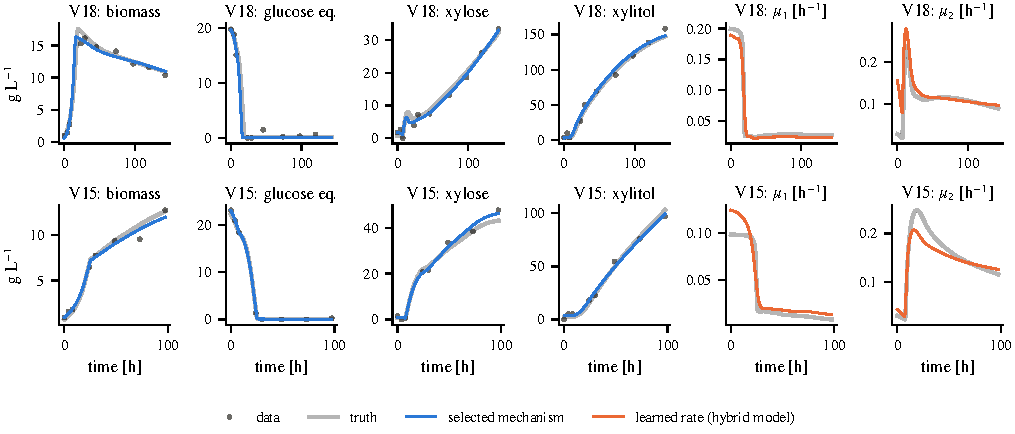
\includegraphics[width=\textwidth]{figs/c2_virtual.pdf}
\caption{Case study 2, virtual runs V18 (top, true mechanism M31) and V15 (bottom, true mechanism M28), first noise realisation: measurements, true trajectories and the trajectories of the selected mechanism, and the specific rates $\mu_1$ and $\mu_2$ learned by the hybrid model compared with the true ones.}
\label{fig:c2virtual}
\end{figure*}

Symbolic regression produced no false discoveries (\VeighteenFD{} and \VfifteenFD{} accepted laws). In \VirtSRexp{} of the \VirtSRn{} analyses, the best proposed conversion law contained the exponential product-inhibition term, and in \VirtSRexpMonod{} it was exactly $\mu_2=a\,S_2\,e^{-P/K}/(b+S_2)$, which reproduces the hyperbolic product inhibition of M28 and M31 within the noise over the observed range of $P$. On V18 it ranks marginally ahead of M31 (median $\Delta\BIC=\VeighteendBICmed$, never below \VeighteendBICmin), because it describes the same behaviour with one parameter fewer; on V15 it ties with M28 (median \VfifteendBICmed). The best proposed law included a death term where the generating mechanism has one and omitted it where it does not in \VirtSRdeath{} of the \VirtSRn{} analyses. Both are far from the acceptance threshold: an alternative functional form of the same mechanism is proposed, compared and correctly not accepted.

\subsection{Real runs analysed individually}\label{sec:c2:real}
For the real runs the measurement errors are unknown, and the candidates were ranked by the profile-likelihood criterion of Eq.~\eqref{eq:bic_profile} with one error standard deviation per species. Table~\ref{tab:c2real} and Fig.~\ref{fig:c2weights} summarise the selection and Fig.~\ref{fig:c2real} shows the fits. Each run was analysed in \BCfifteenMinutes--\BCtwelveMinutes\,min, with the candidates refined in parallel.

\begin{table*}[width=\textwidth,cols=9,pos=t]
\caption{Case study 2, real runs: number of measurements, selected mechanism and shortlist (BIC weights in parentheses), residual standard deviations of the selected mechanism [g\,L$^{-1}$], and BIC difference between the best symbolic-regression law and the selected mechanism (negative: the proposed law is preferred).}\label{tab:c2real}
\begin{tabular*}{\tblwidth}{@{}LCLLCCCCC@{}}
\toprule
Analysis & $n$ & Selected & Shortlist & $X$ & $S_1$ & $S_2$ & $P$ & $\Delta\BIC_{\mathrm{SR}}$ \\
\midrule
\inputtab{generated/tab_c2_real.tex}
\bottomrule
\end{tabular*}
\end{table*}

\begin{figure}
\centering
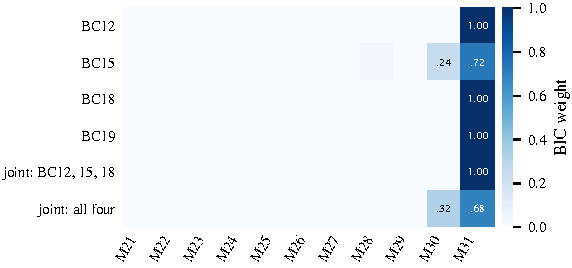
\includegraphics[width=\linewidth]{figs/c2_real_weights.pdf}
\caption{Case study 2, real runs: BIC weights of the eleven library mechanisms for each run analysed alone and for the joint analyses.}
\label{fig:c2weights}
\end{figure}

\begin{figure*}
\centering
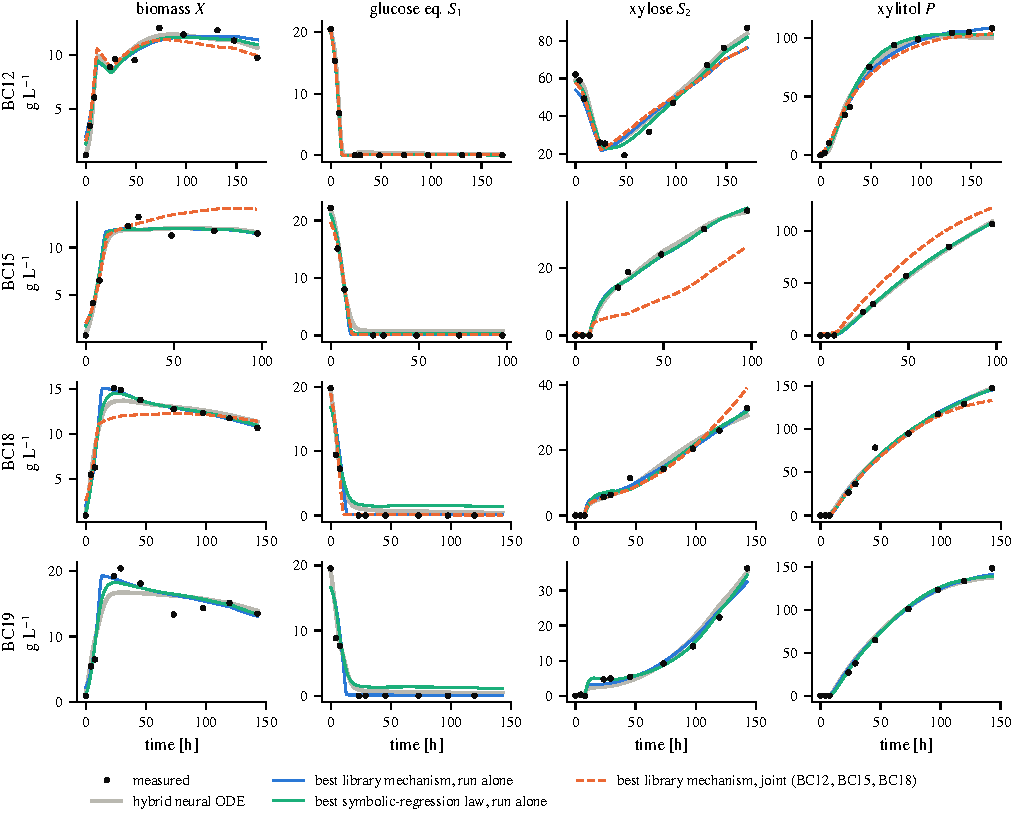
\includegraphics[width=\textwidth]{figs/c2_real.pdf}
\caption{Case study 2, real runs BC12, BC15, BC18 and BC19 (rows): measurements, hybrid neural ODE, best library mechanism and best symbolic-regression law fitted to each run alone, and best library mechanism fitted to BC12, BC15 and BC18 jointly.}
\label{fig:c2real}
\end{figure*}

M31 was selected for every run, with a weight of \BCtwelveW{} for BC12, \BCeighteenW{} for BC18 and \BCnineteenW{} for BC19, and \BCfifteenW{} for BC15, where M30, the same mechanism without death, took most of the remaining weight. The four runs therefore agree on the qualitative mechanism: xylitol formation slows down because both xylose and xylitol inhibit it, and the biomass declines through first-order death during the long production phase. It is consistent with the hybrid model, which learned death rates of 0.013--0.020\,h$^{-1}$ and a conversion rate that declines during the feed phase in BC12, BC18 and BC19 and stays nearly constant in BC15. The residual standard deviations are 1--10\,\% of the ranges of the measured species, with two systematic deviations visible in Fig.~\ref{fig:c2real}. First, the fitted initial biomass exceeds the first measurement by \BCtwelveDXzero, \BCfifteenDXzero, \BCeighteenDXzero{} and \BCnineteenDXzero\,g\,L$^{-1}$ in the four runs, close to the bound of the initial states. This is a limitation shared by all candidates: with a single growth substrate, the model cannot represent the batch phase, in which the yeast grows fast on glucose and then more slowly on the ethanol it produced, and it compensates through the initial biomass. Second, in BC12, the only run with xylose in the batch medium, M31 misses the minimum of the xylose concentration by up to 11\,g\,L$^{-1}$.

The parameter values differ between the runs (Table~\ref{tab:c2params}), and several are poorly determined. The constants of the conversion rate trade off against each other: $K_{S_2}$ lies far above the observed xylose concentrations in three runs, while $K_{SI_2}$ varies between 0.3 and 13\,g\,L$^{-1}$; and $K_{S_1}$ reached its upper bound in two runs. The rates implied by the fits are more comparable than the constants: evaluated at a common state ($S_2=30$ and $P=50$\,g\,L$^{-1}$), the conversion rate of the selected mechanism is \BCtwelveMuRef, \BCfifteenMuRef{} and \BCeighteenMuRef\,h$^{-1}$ for BC12, BC15 and BC18, but only \BCnineteenMuRef\,h$^{-1}$ for BC19, the run supplemented with corn steep solids.

\begin{table*}[width=\textwidth,cols=7,pos=t]
\caption{Case study 2: parameters of M31 fitted to each real run alone and to groups of runs jointly with shared parameters.}\label{tab:c2params}
\begin{tabular*}{\tblwidth}{@{}LCCCCCC@{}}
\toprule
Parameter & \inputtab{generated/tab_c2_real_params_head.tex} \\
\midrule
\inputtab{generated/tab_c2_real_params.tex}
\bottomrule
\end{tabular*}
\end{table*}

\subsection{Real runs analysed jointly}\label{sec:c2:joint}
In case study~1, fitting several runs jointly resolved the ambiguity of single runs. That required the runs to share their kinetics, which held by construction. For real runs it is a hypothesis, and it can be tested with the same criterion: the BIC of a joint fit with one set of kinetic parameters is compared with the BIC of separate fits of the same runs, both evaluated with one error standard deviation per species pooled over the runs (Table~\ref{tab:c2shared}). Because the separate fits were obtained with run-specific error weights, their pooled criterion is an upper bound on its optimum, and the comparison is conservative with respect to separate kinetics.

\begin{table}[width=\linewidth,cols=5,pos=t]
\caption{Case study 2: shared versus run-specific kinetics. BIC of M31 fitted jointly with shared parameters minus BIC of M31 fitted to each run separately, both with one error standard deviation per species pooled over the runs (positive: run-specific parameters are preferred); $k$ counts the kinetic parameters.}\label{tab:c2shared}
\begin{tabular*}{\tblwidth}{@{}LCCCC@{}}
\toprule
Runs & $n$ & $k$ shared & $k$ separate & $\Delta\BIC$ \\
\midrule
\inputtab{generated/tab_c2_shared.tex}
\bottomrule
\end{tabular*}
\end{table}

Joint fitting again selected M31: with a weight of \JointThreeW{} for the three runs in yeast extract--peptone medium (BC12, BC15 and BC18) and of \JointFourW{} for all four runs, with M30 taking the rest (Table~\ref{tab:c2real}, Fig.~\ref{fig:c2weights}). The shared parameters, however, do not describe the runs equally well. In the joint fit of BC12, BC15 and BC18, the residual standard deviations of xylose and xylitol in BC15 rise from about 1\,g\,L$^{-1}$ in its individual fit to 9 and 12\,g\,L$^{-1}$ (Fig.~\ref{fig:c2real}, dashed lines), and the fitted initial biomass of the four-run fit lies 1.8--2.9\,g\,L$^{-1}$ above the first measurements, at the bounds of the initial states. Accordingly, run-specific parameters were preferred for every group of runs tested (Table~\ref{tab:c2shared}), with $\Delta\BIC=\SharedThree$ for the three runs in the same medium and $\Delta\BIC=\SharedTwo$ for BC15 and BC18, the two runs with the most similar operation. The real runs therefore share a mechanism but not its parameter values, and the differences are larger than their measurement errors.

This has a direct consequence for the symbolic regression. For the joint analyses the best proposed laws were preferred to M31 beyond the acceptance threshold ($\Delta\BIC=\JointThreeSRdBIC$ and $\JointFourSRdBIC$; Table~\ref{tab:c2sr}). Both have the same structure, a Monod-type conversion rate with an additional numerator term that decays exponentially with xylitol and a combined inhibition term $PS_2^2$ in the denominator, and their additional terms may absorb part of the differences between the runs: in the three-run fit, for instance, the exponential term has fallen to 10\,\% at 3\,g\,L$^{-1}$ xylitol and only describes a transient at the start of the feed. A law that wins because the model with shared parameters is misspecified is exactly what the adequacy condition of the acceptance rule is meant to reject; without known measurement errors it cannot be applied, and these laws were not accepted.


\subsection{Symbolic regression on the real runs}\label{sec:c2:sr}
Table~\ref{tab:c2sr} lists the best law proposed by the symbolic regression for each analysis; the joint analyses are discussed in Section~\ref{sec:c2:joint}. For the individual runs no proposed law met the acceptance threshold. For BC12 and BC19 the best proposed law was preferred to M31 ($\Delta\BIC=\BCtwelveSRdBIC$ and $\BCnineteenSRdBIC$), close to but not beyond the threshold, for BC15 the two tie, and for BC18 M31 is clearly better. Moreover, the adequacy condition cannot be evaluated without known measurement errors, so on real data even a law that crossed the threshold would be reported as a candidate for further experiments rather than accepted into the library. The proposed laws nevertheless carry information. For every run they include first-order death and describe the decline of the conversion by exponential rather than hyperbolic product inhibition, $\mu_2\propto e^{-P/K}$ with $K$ between 67 and 313\,g\,L$^{-1}$ xylitol. For BC12 the regression adds strong substrate inhibition, $\mu_2\propto S_2e^{-P/K}/(1+S_2^2/K_I)$, and halves the residual standard deviation of xylose relative to M31 (3.6 against 6.7\,g\,L$^{-1}$; Fig.~\ref{fig:c2real}). And the growth laws proposed for BC18 and BC19 are of first order in the glucose equivalent over the observed range, which, together with $K_{S_1}$ at its upper bound, indicates that growth on the lumped substrate saturates more weakly than the library assumes.

\begin{table*}[width=\textwidth,cols=5,pos=t]
\caption{Case study 2, real runs: best laws proposed by symbolic regression and their BIC difference to the best library mechanism. Concentrations in g\,L$^{-1}$, rates in h$^{-1}$; terms that contribute less than 1\,\% of the numerator or denominator over the measured states are omitted.}\label{tab:c2sr}
\begin{tabular*}{\tblwidth}{@{}LLLCC@{}}
\toprule
Analysis & $\mu_1$ & $\mu_2$ & Death & $\Delta\BIC$ \\
\midrule
\inputtab{generated/tab_c2_real_sr.tex}
\bottomrule
\end{tabular*}
\end{table*}

